\documentclass{tufte-handout}

\usepackage{../CommonLatexPackages/fall2018_preamble_v1.0}
\fancypagestyle{firstpage}

{\rhead{Day 6 \linebreak \textit{Version: \today}}}

\title{Day 6: The RANSAC Algorithm and Finding Lines}
\author{Quantitative Engineering Analysis}
\date{Spring 2019}

\begin{document}

\maketitle
\thispagestyle{firstpage}

\section{Schedule}
\begin{itemize}
\item 0900-0915: Quiz
\item 0915-0950: Debrief on Using Experimental Data
\item 0950-1020: RANSAC
\item 1020-1035: Coffee
\item 1035-1125: Pseudo-coding
\item 1125-1215: Implementation
\item 1215- 1230: Preview
\end{itemize}

\section{Quiz}

\section{Benchmark Quiz [15 mins]}
\be
\item The diagram at the right shows a contour map of a two dimensional function, $f(x,y)$, along with points marked A through E.

\begin{marginfigure}
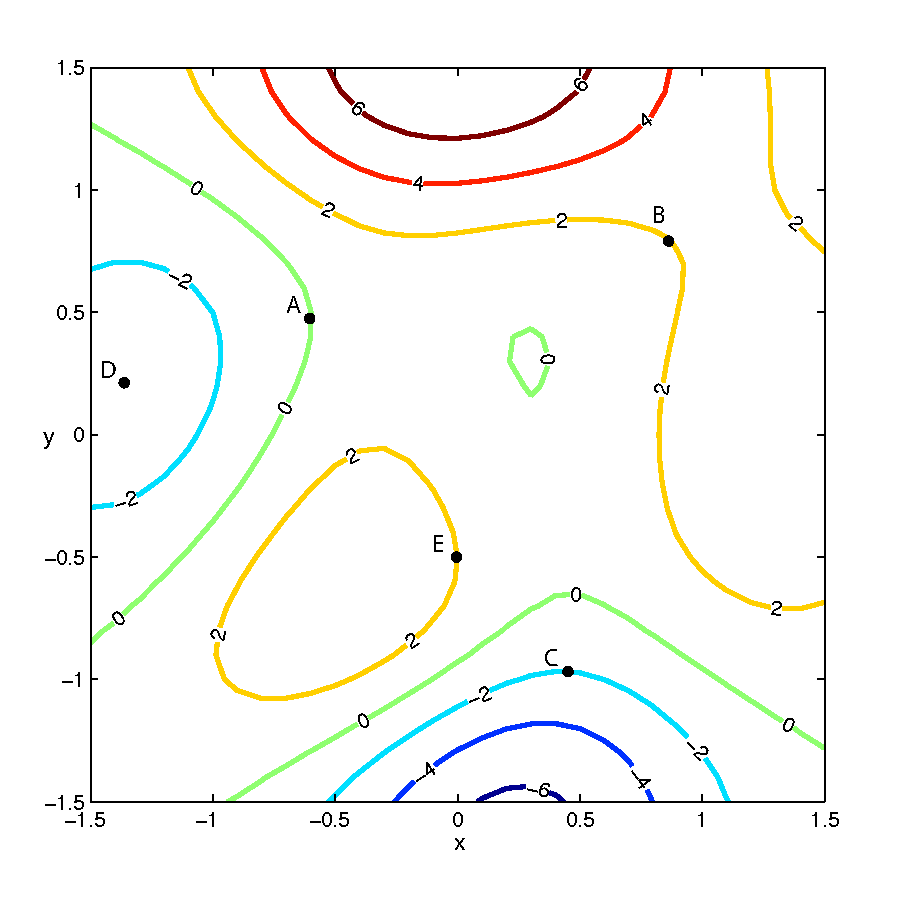
\includegraphics[width=3in]{Figures/ContourExampleForQuiz.pdf}
\end{marginfigure}
\be
\item At which point is $f(x,y) \approx 0$?
\item At which point is $|\nabla f(x,y)| \approx 0$?
\item At which point is $|\nabla f(x,y)|$ largest?
\item At which point is $\frac{\nabla f(x,y)}{|\nabla f(x,y)|} \approx +\hat{i} \;$?
\item At which point does the determinant of the Hessian of $f(x,y)$ most clearly appear to be positive?
\ee

\item True or false...
\be
\item If the magnitude of the gradient is zero, you must be at a max or a min.
\item Regardless of starting point, gradient ascent will always find the global maximum of a multivariable function.
\item Gradient ascent always follows the shortest path to a maximum.
\item If $f(x,y,z)$ is a scalar function in three dimensions, $\nabla f(x,y,z)$ is also a scalar function in three dimensions.
\item The $\nabla$ operator is sometimes referred to as the ``upside down triangle'' by students who wish to irritate professors.
\ee

%\item In the second method of gradient ascent, you follow the initial direction of the gradient (call it $\hat{t}_i$) until...
%\be
%\item $\nabla f \cdot \hat{t}_i > 0$
%\item You reach a minimum of $f$ along the line
%\item $\nabla f \perp \hat{t}_i$
%\item Your pencil goes off the page
%\ee

\item Assume point D is a minimum.  If you started a gradient ascent at point D, approximately where would you end up?
\be
\item Point D
\item Somewhere in the vicinity of $(0,1.5)$
\item Somewhere in the vicinity of $(-0.5,-0.5)$
\item Somewhere in the vicinity of $(0.25,-1.6)$
\item You cannot tell with the information provided.
\ee

\item What is the cartesian point (12,5) in polar coordinates?
\be 
\item r = 12, $\theta=5^\circ$
\item r = 13, $\theta=22.6^\circ$
\item r = 13, $\theta=67.4^\circ$
\ee

\item {\bf atand} in MATLAB returns angles between -90 degrees and 90 degrees. Assuming we want to return angles between 0 degrees and 360 degrees, match the quadrant and how to treat {\bf atand}. You may wish to review "quadrants" from trigonometry.
\begin{center}
\begin{tabular}{ |c|l| } 
 \hline
 Quadrant & {\bf atand}  \\
 \hline
 \hline
I & (a) Add 180$^{\circ}$ to the function value\\
II & (b) Subtract 180$^{\circ}$ from the function value\\
III & (c) Add 360$^{\circ}$ to the function value\\
IV & (d) Use the value from the {\bf atand} function\\
 \hline
\end{tabular}
\end{center}

\ee


\section{Debrief on Experimental Data Analysis [35 minutes]}

In both the mapping of the Bridge of Doom and when experimenting with the LIDAR data, we were working with real experimental sensor data and trying to extract information from this data.  Real data is, as you have probably noticed, inherently messy in a variety of different ways.  In the course of mapping the Bridge of Doom and the initial LIDAR assignment, there were several examples of common data analysis issues which you needed to deal with.  For this debrief, we'd like you to consider the following list of data analysis issues.  Working with a partner at the boards, create a table.  For each entry in this list, draw a sketch representing the concept, give an example of this issue from your work this week, indicate how you identify the issue, and how you deal with the issue. Lastly, can you come up with another example of this from another context?  Some of these are closely related to each other, also this is nowhere near an exhaustive list:  please feel free to add to it.

\begin{itemize}
\item Timing:time origin
\item Timing:sampling rate
\item Coordinate system/origin
\item Scatter/statistical error
\item Outliers
\item Systematic error
\item Measurement device limitations
\item Accuracy
\item Precision
\end{itemize}

\section{RANSAC [30 minutes]}
Today we'll be learning a technique for optimization in the presence of outliers. The algorithm is called Random Sample Consensus, RANSAC for short, and it has applicability to a wide variety of problems in robotics and computer vision.  In The Gauntlet\texttrademark~we'll be using it to find lines in laser scan data even when multiple structures are present (e.g., multiple walls, lines and circles).

By the end of this activity, you should be comfortable with:
\begin{enumerate}
\item Using the RANSAC algorithm to find a line in a laser scan.
\item Finding multiple lines using the RANSAC algorithm.
\end{enumerate}

\subsection{Motivating Example}
\begin{figure}
\begin{center}
\includegraphics[width=.8\linewidth]{Figures/naivelinefit-eps-converted-to.pdf}
\end{center}
\caption{The lines of best fit as computed by linear regression and PCA.  Due to the mixed structures in the data, the results are very poor.\label{fig:naivefit}}
\end{figure}

In the overnight, you applied line fitting techniques to four different laser scans.  The linear regression method worked well in some cases, but it had some clear shortcomings (e.g., when the scan points were oriented vertically).  The PCA algorithm was able to overcome some of these limitations, however, there were cases when even PCA failed.  For instance, Figure~\ref{fig:naivefit} shows the results of applying both linear regression and PCA to \href{https://drive.google.com/file/d/1bDu-QAPmyNc4SRFicWCiNtEOgpAmaB_g/view?usp=sharing}{scan4.mat}.  Due to the fact that there are outliers (i.e. points that do not lie on the line), both linear regression and PCA find lines that do not correspond at all to the line clearly visible in the scan.

We can conclude from this example that the methods of line fitting that we've learned thus far are effective yet brittle (i.e. they fail when conditions aren't ideal).  Motivated by this observation, today we'll be learning how to use the RANSAC algorithm to filter outliers \emph{before} applying one of the line fitting methods you explored in the overnight.

\subsection{Robust Optimization and the RANSAC Algorithm}\label{sec:ransac}
The mathematical field of robust optimization provides us with techniques for optimizing functions (such as $MSE$) that are robust in the presence of outliers.  Today, you'll explore a very powerful technique for robust optimization called \href{https://en.wikipedia.org/wiki/Random_sample_consensus}{Random Sample Consensus} (or RANSAC for short).  The algorithm works by choosing a small subset of data points to fit a model, determining whether or not a significant proportion of the data is consistent with the fitted model, and then repeating this process until a satisfactory model is found.  For instance, let's suppose we want to find a line in this laser scan.

\begin{center}
\includegraphics[width=0.6\linewidth]{Figures/mixedscan}
\end{center}

The RANSAC algorithm starts by randomly choosing a minimal subset of data points required to define a line (which of course is 2).  Given these 2 points, we define our candidate line as the line that passes through both of those points (this is our ``model'').  Next, we divide \emph{all} of the points in our laser scan into two groups.  The first group, called \emph{inliers}, consists of points in the laser scan that are sufficiently close to our candidate line.  The second group of points, called \emph{outliers}, consists of points in the laser scan that are far from the candidate line.  We are free to choose the notion of what it means to be close or far from our candidate line.  Based on our experience in the overnight, the perpendicular distance seems like a reasonable choice to measure the closeness of a point to a line (recall that this is what PCA uses).  Therefore, we'll use the perpendicular distance as a metric for deciding whether a point is an inlier or an outlier.  Figure~\ref{fig:mixedscansubset} shows an example of applying this procedure.  The inliers are marked in either white (for the two points used to make the line) or blue.  The inliers are the points that fall within a perpendicular distance $d$ from the line ($d$ is a threshold value that you specify to RANSAC).  The outliers (those that fall outside of a distance $d$ of the line) are marked in red.  While the line defined by the two randomly chosen points results in some inliers, the number of inliers (4 including the points used to make the line) is perhaps not as large as it could be.

\begin{marginfigure}
\begin{center}
\includegraphics[width=\linewidth]{Figures/mixedscansubset}
\end{center}
\caption{The white points represent the randomly chosen subset of two points to define the line.  The solid line passing through them is the resultant line.  The two dashed lines correspond to the inlier threshold (defined by measuring a specified distance $d$ perpendicularly from the line).  The points that are inliers are marked in blue and the outliers are red.\label{fig:mixedscansubset}}
\end{marginfigure}

\begin{marginfigure}
\begin{center}
\includegraphics[width=\linewidth]{Figures/mixedscansubsetmax}
\end{center}
\caption{The white points represent the randomly chosen subset of points and to define the line.  The solid line passing through them is that resultant line.  The two dashed lines correspond to the inlier threshold (defined by measuring a specified distance $d$ perpendicularly from the line).  The points that are inliers are marked in blue and the outliers are red.\label{fig:mixedscansubsetmax}}
\end{marginfigure}

Next, we choose a new random set of 2 points, define the line passing through those points as our candidate line, and determine inliers and outliers.  If this new candidate line results in more inliers than the first one we tried, we save the line for later.  We repeat the procedure (choosing two random points, determining inliers, and testing to see if the number of inliers is the highest we've found so far) $n$ times, where $n$ is a parameter that you specify to the RANSAC algorithm.  If all goes well, one of these $n$ lines results in something like Figure~\ref{fig:mixedscansubsetmax}.  For the randomly chosen points shown in the figure, the number of inliers is 7 which looks to be about as good as we can do with this scan data.

As a final consideration, in the case of fitting lines to laser scan data, we want to be able to determine not just where the lines are in the scan, but also where the lines begin and end.  This is crucial since the lines we are finding correspond to things like the beginning and end of walls or obstacles.  There are a few ways to approach this task, and we'd like you to come up with your own method as part of today's activities.  We are certainly here to scaffold this, but wrestling with this a bit will help to build your intuition about the geometry of the problem.

\section{Coffee Break [15 minutes]}

\section{Converting from Intuition to Pseudocode [50 minutes]}
Let's take stock of where we are.  You should now have a pretty good idea about how RANSAC works on a conceptual level.  Next, you'll be working to take this intuition and convert it into pseudocode.

When writing pseudocode it helps to start by stating your high-level conceptual understanding of how to solve the problem, and then, work towards progressively more concrete statements of how to solve the problem.  Motivated by this idea, here's a possible procedure you can use with your partner to generate pseudocode.

\begin{enumerate}
\item \textbf{Clear up conceptual misunderstandings:} You just read through some text that described the RANSAC algorithm.  Were there any parts that didn't make sense at a conceptual level?  If so, make sure you work through these with your partner.  If you can't figure out one of your questions, let us know!  We're here to help.
\item \textbf{Simulate the algorithm:} at the whiteboard, simulate the steps that RANSAC would go through to find a line in a laser scan.  You can do this through a combination of pictures (like the ones in Figure~\ref{fig:mixedscansubsetmax}) and explanatory text (e.g., select points at random).  As you go through this process you may find that you don't understand some of the details as well as you thought.  This is another chance to ask for help from the teaching team.
\item \textbf{Write out the major steps:} Next, write the sequence of major steps the algorithm should perform.  By this point your descriptions should be getting more precise (although not necessarily more detailed).  Deciding how big to make each step is a bit of a balancing act.  You want to avoid sequences such as ``1.  Do the thing 2.  ??? 3.  Profit'', but you certainly don't want to have a 25 step process.  Shoot for something on the order of 5-7 steps.  Each of these steps can later be subdivided into smaller pieces.
\item \textbf{Figure out your functions:} the major steps you've defined can be thought of as the functions that you will write to implement your algorithm.  For instance, you may have come up with a step called ``compute inliers and oultiers''.  The fact that you identified this as a major step for your algorithm suggests that making a function that performs this computation is probably a good idea.  At the whiteboard write out a list of the functions you will create when implementing RANSAC.  Make sure to describe what each of these functions expects as input, what it will generate as output, and what it does.
\item \textbf{Write your pseudocode:}  Next, write pseudocode for each of the functions you've identified as well as  pseudocode that stitches these functions together to implement RANSAC.  Your pseudocode should be written in natural language (avoid using actual MATLAB syntax in your pseudocode), yet precise enough that there is little ambiguity about how it could be translated into actual MATLAB code.  To better make this last point, here are two different potential ways to write pseudocode for finding the maximum element in a list of values.

\begin{verbatim}
Input: a list of numbers L
for each number x in the list L
    if x is the highest value so far
        remember x
return the highest value we found
\end{verbatim}
This pseudocode has some good properties.  It is written in natural language and it specifies the inputs of the function.  On the negative side there is still a good deal of ambiguity here.  How do I test if ``x is the highest value so far''?  How do I ``remember x''?  Here's a version that improves the pseudocode in this respect.

\begin{verbatim}
Input: a list of numbers L
initialize a variable called maxval to the value negative infinity
for each number x in the list L
    if x is greater than maxval
        assign the value of x to maxval
return the variable maxval
\end{verbatim}

This new version of the pseudocode can be unambiguously translated to a computer program.

\end{enumerate}

\begin{enumerate}[series=exercises, label=\textbf{Exercise} (\arabic*)]
\item Write pseudocode to implement the algorithm described in Section~\ref{sec:ransac}.  Your pseudocode should be capable of going from a polar coordinate representation of a laser scan to the endpoints, in Cartesian space, of a line segment that corresponds to a line in the laser scan.
\end{enumerate}

\section{Implementing Your Algorithm [50 minutes]}

In this section you'll be translating your pseudo-code into MATLAB.

\begin{enumerate}[resume=exercises, label=\textbf{Exercise} (\arabic*)]
\item Implement RANSAC using the pseudocode you wrote in the previous exercise.  Test your algorithm on the data in \href{https://canvas.instructure.com/courses/1096977/files/50482786/download?wrap=1}{scan4.mat}.  As a suggestion, you should define a top-level function called \emph{robustLineFit} that takes as input a polar representation of the laser scan, the threshold $d$ to use to determine whether a scan point is an inlier, and $n$ the number of random lines to try.  Once you've implemented your algorithm, experiment with $d$ and $n$ to understand their effect.
\end{enumerate}

\vspace{1em}
\begin{myboxi}
Debugging and implementation tips:
\begin{enumerate}
\item Visualize, visualize, visualize.  For instance, make sure your procedure for determining inliers is correct, you should plot the fitted line, the inliers, and the outliers.  Make sure to use different colors to plot the inliers versus outliers.
\item Develop incrementally.  Build your program bit by bit.  Experiment in the command window before writing code in your MATLAB script.
\item Set breakpoints.  This can be accomplished by either using the \emph{keyboard} statement or by creating a stop sign by clicking to the left of the line of MATLAB code.  These breakpoints are particularly useful in two situations.  The first situation is obvious -- when attempting to debug code.  The second situation is when you are about to write an intricate section of code.  In this case, set the breakpoint where the code will eventually go.  Run your existing (but incomplete) code.  When MATLAB stops at the break point, you can prototype your solution in the command window before adding it into your script.
\end{enumerate}
\end{myboxi}

If all has gone well, you should have a beautiful line segment fit to the data in \emph{scan4.mat}.  Unfortunately for you, The Gauntlet\texttrademark~is a bit more complicated than the Chamber of Emptiness\texttrademark.  Next you'll be updating your code to find multiple lines.

\begin{enumerate}[resume=exercises, label=\textbf{Exercise} (\arabic*)]
\item First, write pseudocode to find multiple lines in a laser scan.  When doing this you should HEAVILY leverage what you did in exercise 3.  For instance, if you have a function called \emph{robustLineFit} which takes a scan and computes the best fitting line segment, you can call it repeatedly to find multiple lines.  Specifically, each time you call your \emph{robustLineFit} code, you'll determine a line segment in scan.  After determining a line segment, you should remove the inlier points for that line segment from the scan data.  By removing these scan points each subsequent line you find will consist of points that were outliers with respect to the lines you previously found.  Implement your approach and try it on the data stored in \href{https://drive.google.com/file/d/1GDjJZEugLjlzMgyxxT4KXzV7mgYv3kvI/view?usp=sharing}{playpensample.mat}.
\ee

\vspace{1em}
\begin{myboxi}
Debugging and implementation tips:
\begin{enumerate}
\item In order to write this in a sane fashion, your functions will need to be solid.  Make sure you are confident in each function before building on it.
\item You may consider modifying your \emph{robustLineFit} to return multiple pieces of information (instead of just the line segment of best fit).  For instance, if you return the inlier points and outliers points separately your life will be a lot easier.  If you're not familiar with returning multiple outputs from a MATLAB function, see \href{https://www.mathworks.com/help/matlab/ref/function.html}{this page}.
\end{enumerate}
\end{myboxi}

If all went well you should now be finding all the walls in a fairly complex laser scan.  You may have noticed some warts in the lines that your code finds.  The biggest issue is that the line segments that are found sometimes have large gaps in them.  This causes you to find lines that span across gaps in the environment.  Later in the challenge you'll be using these line segments to determine a path through the environment, so it is important that the gaps are not covered over by spurious lines.

\vspace{1em}
\begin{enumerate}[resume=exercises, label=\textbf{Exercise} (\arabic*)]
\item Modify your \emph{robustLineFit} code to avoid fitting line segments with large gaps.  To do this, define a procedure for computing the largest gap in a candidate line segment.  Start out by working on the board to build intuition, and only when you have a good sense of how to solve the problem, implement things in MATLAB.
\ee

\section{Preview of the Overnight [15 minutes]}


\end{document}
